\chapter{Semantics}
\label{semantics}
\section{Abstract Syntax for Ezuino}
Now that we have made the syntax for the Ezuino language, the next step is to construct semantics for the programming language. This chapter will describe the semantic rules of the Ezuino language.
Before we can start on semantics, an overview is needed to provide an overview of the short names in each semantic. This is provided by 
Table \ref{syntactic-categories}. 
The context free grammar is interesting when analyzing a language's syntax, as the abstract syntax only describes the structure of the linguistic constructs. The abstract syntax for the Ezuino language can be found in  Table \ref{abstract-syntax}.
\begin{table}[H]
\centering
\begin{tabular}{|c|c|}
\hline
\textbf{Syntax} & \textbf{Definition}   \\ \hline
!TE              & Type Environment      \\ \hline
$D_v$           & Variable Declarations \\ \hline
$D_f$           & Function Declarations \\ \hline
S               & Statements            \\ \hline
T               & Type                  \\ \hline
a               & Arithmetic expressions\\ \hline
b               & Boolean expressions   \\ \hline
n               & Numeral literal(Integer or Double) \\ \hline
e               & Expression            \\ \hline
$\beta$         & Boolean literal       \\ \hline
x               & Variables             \\ \hline
$f$             & Function Names        \\ \hline
P               & Parameters            \\ \hline
C               & Block structure       \\ \hline
param           & Parameters            \\ \hline
r               & Return statement      \\ \hline
\end{tabular}
\caption{Syntactic categories for Ezuino}
\label{syntactic-categories}
\end{table}

\begin{longtable}[c] { r c c }
  \label{abstract-syntax}
  \centering
  
  \(a\) & \(::=\) & \(\ n\ |\ x\ |\ a_1*a_2\ |\ a_1 + a_2\ |\ a_1 - a_2\ |\ a_1 / a_2\ |\ -a \) \\
    &  & \\
  
  \(b\) & \(::=\) & \(\ \beta \ |\ !b\ |\ x\ |\ b_1 = b_2\ |\ b_1 != b_2\ |\ b_1\ AND\ b_2\ |\ b_1\ OR\ b_2\ \) \\
    &  & \\
  
  \(e\) & \(::=\) & \(\ (e)\ |\ f(param)\ |\ a\ |\ b\ \) \\
    &  & \\

  \(S\) & \(::=\) & \(x := e\ |\ if(e)\ C_1\ else\ C_2\ |\ while\ (e)\ C\ |\ return\ e\ |\ return\ |\ S_1\ S_2\ |\ f(param) |\ \epsilon\ \) \\
    &  & \\

  \(D_f\) & \(::=\) & \(func\ T\ f(P)\ C \) \\
    &  & \\

  \(D_v\) & \(::=\) & \( T\ x\ |\ T\ x\ D_v\ |\ \epsilon \) \\
    &  & \\

  \(P\) & \(::=\) & \( T\ x\ |\ T x,\ P\ |\ \epsilon \) \\
    &  & \\

  \(param\) & \(::=\) & \( e\ |\ e,\ param\ |\ \epsilon \) \\
    &  & \\

  \(prog\) & \(::=\) & \( D_v\ S \) \\
    &  & \\

  \(T\) & \(::=\) & \( int\ |\ double\ |\ boolean\ |\ string \) \\
    &  & \\

  \caption{Abstract syntax for Ezuino}
\end{longtable}

\section{Structural Operation Semantics}
The operational semantics are the rules that give our syntax meaning, and without them it would be impossible to make a working language, as a given syntax wouldn't have a clearly defined functionality. For this reason, we will define the operational semantics in this section.

There are 2 different ways of describing semantics of a language. Big-step semantics and small-step semantics. While they are equivalent, there are some advantages and disadvantages to both of them. The big-step semantics evaluates the whole expression from the start to the end expression. Small-step semantics may only evaluate part of the expression one step at a time. The disadvantage of small-step semantics is that it can be daunting to both write and read.

We have decided to make our operational semantics a small-step semantic, as a small-step semantic ruleset is easier to extend in the case of a new feature compared to a big-step semantic ruleset. This means that it would be possible to add parallelity, if we realize that we need it at a later date.

\subsection{Environment-Store Model}
One of the ways we can describe how the Ezuino compiler must handle and store variables, we must just the Environment Store Model (ESM). There are differnet mechanism inside the ESM, and some we will go through the essentials before starting on the semantics. First, we have the location, which marks the location of every variable value in the program. The location keeps track of a variable in the environment $env_v$.
To continue with the ESM, we got the partial function named Store (Sto), which for an instance of the program binds its storage location to values, which are contained within. An example of this, is that if we want to find the value of a specific variable, in this case named x, we write $"sto \  env_v \ x"$.
Next we have the run-time s tack named envl. The runtime stack is a list of pairs ($env_v$, $env_p$).
On figure \ref{evnstoreexmp}, the ESM can be reviewed.
\begin{figure}[H]
\centering
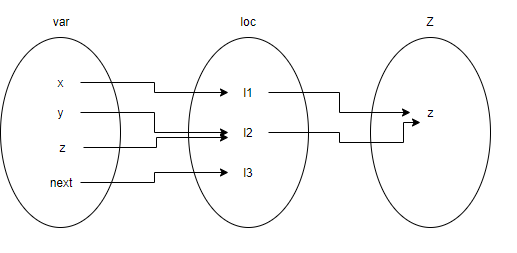
\includegraphics[scale=0.75]{figures/evnstore.png}
\caption{Environment Store Example}
\label{evnstoreexmp}
\end{figure}

\subsection{Arithmetic Expressions}
In the following table, it should be noted that most transitions will be on the form \( \langle envl, sto, a \rangle \Rightarrow_e \langle envl', sto', v \rangle \). This is supposed to be read as "By evaluating a in accord with the runtime stack and the store like an expression, a is evaluated to the value v, and the runtime stack and store is updated

\begin{longtable}[c] { r c }
  \centering
  
  [VAR] & \( envl, sto \vdash x \Rightarrow_e v \) \\
  & if \(env_v x = l \) \\
  & and \(sto \ l = v \) \\
  & where \(envl = (env_v, env_p) : envl' \) \\
  &  \\

  [DCL] & \( 
    \dfrac{ \langle D_V, envl[x \mapsto l][next \mapsto \text{new} \ l], sto \rangle \Rightarrow_{DV} \langle envl', sto \rangle}
    { \langle T x, envl, sto \rangle \Rightarrow_{DV} \langle envl', sto \rangle } \) \\
  & \\

  [PARENT-1] & 
    \( \dfrac { \langle e, envl, sto \rangle \Rightarrow_e \langle e', envl', sto' \rangle }
      { \langle (e), envl, sto \rangle  \Rightarrow_e \langle (e'), envl', sto' \rangle } \) \\
  & \\

  [PARENT-2] & 
    \( \langle (v), envl, sto \rangle \Rightarrow_e \langle v, envl, sto \rangle \) \\
  & \\

  [PLUS-1] & 
    \( \dfrac { \langle e_1, envl, sto \rangle \Rightarrow_e \langle e_1', envl', sto' \rangle )}
      {\langle e_1 + e_2, envl, sto \rangle \Rightarrow_e \langle e_1' + e_2, envl', sto' \rangle } \) \\
  & \\

  [PLUS-2] & 
    \( \dfrac { \langle e_2, envl, sto \rangle \Rightarrow_e \langle e_2', envl', sto' \rangle }
      {\langle v_1 + e_2, envl, sto \rangle  \Rightarrow_e \langle e_1 + e_2', envl', sto' \rangle } \) \\
  & \\

  [PLUS-3] & 
    \( \langle v_1 + v_2, envl, sto \rangle \Rightarrow \langle v, envl, sto \rangle \) \\
  & where \( v = v_1 + v_2\) \\
  & \\

  [MINUS-1] & 
    \( \dfrac { \langle e_1, envl, sto \rangle \Rightarrow_e \langle e_1', envl', sto' \rangle }
      {\langle e_1 - e_2, envl, sto \rangle \Rightarrow_e \langle e_1' - e_2, envl', sto' \rangle } \) \\
  & \\

  [MINUS-2] & 
    \( \dfrac { \langle e_2, envl, sto \rangle \Rightarrow_e \langle e_2', envl', sto' \rangle }
      {\langle v_1 - e_2, envl, sto \rangle \Rightarrow_e \langle v_1 - e_2', envl', sto' \rangle } \) \\
  & \\

  [MINUS-3] & 
    \( \langle v_1 - v_2, envl, sto \rangle \Rightarrow \langle v, envl, sto \rangle \) \\
  & where \( v = v_1 - v_2\) \\
  & \\

  [MULT-1] & 
    \( \dfrac { \langle e_1, envl, sto \rangle \Rightarrow_e \langle e_1', envl', sto' \rangle }
      {\langle e_1 * e_2, envl, sto \rangle \Rightarrow_e \langle e_1' * e_2, envl', sto' \rangle } \) \\
  & \\

  [MULT-2] & 
    \( \dfrac { \langle e_2, envl, sto \rangle \Rightarrow_e \langle e_2', envl', sto' \rangle }
      {\langle v_1 * e_2, envl, sto \rangle \Rightarrow_e \langle v_1 * e_2', envl', sto' \rangle } \) \\
  & \\

  [MULT-3] & 
    \( \langle v_1 * v_2, envl, sto \rangle \Rightarrow \langle v, envl, sto \rangle \) \\
  & where \( v = v_1 * v_2\) \\
  & \\

  [DIV-1] & 
    \( \dfrac { \langle e_1, envl, sto \rangle \Rightarrow_e \langle e_1', envl', sto' \rangle }
      {\langle e_1 / e_2, envl, sto \rangle \Rightarrow_e \langle e_1' / e_2, envl', sto' \rangle } \) \\
  & \\

  [DIV-2] & 
    \( \dfrac { \langle e_2, envl, sto \rangle \Rightarrow_e \langle e_2', envl', sto' \rangle }
      {\langle v_1 / e_2, envl, sto \rangle \Rightarrow_e \langle v_1 / e_2', envl', sto' \rangle } \) \\
  & \\

  [DIV-3] & 
    \( \langle v_1 / v_2, envl, sto \rangle \Rightarrow \langle v, envl, sto \rangle \) \\
  & where \( v = \dfrac{ v_1 }{ v_2 } \) \\
  & \\

  [NEGATION-1] & 
    \( \dfrac { \langle e_1, envl, sto \rangle \Rightarrow_e \langle e_1', envl', sto' \rangle }
      {\langle -e_1, envl, sto \rangle \Rightarrow_e \langle -e_1', envl', sto' \rangle } \) \\
  & \\

  [NEGATION-2] & 
    \( \langle -v_1, envl, sto \rangle \Rightarrow \langle v, envl, sto \rangle \) \\
  & where \( v = -v_1 \)\\
  & \\

  [NUM] & 
    \( n \Rightarrow v \) \\
  & \( \text{if } \mathcal{N} [[n]] = v \) \\

  \caption{Small-step semantics for arithmetic expressions}
\end{longtable}

\subsection{Boolean Expressions}
\begin{longtable}[c] { r c }
  \centering
  [NOT-1] & \( 
    \dfrac { \langle e, envl, sto \rangle \Rightarrow_e \langle e', envl', sto' \rangle }
      { \langle !e, envl, sto \rangle \Rightarrow_e \langle !e', envl', sto' \rangle } \)
  \\
  & \\

  [NOT-TRUE] & \( 
    \langle !v, envl, sto \rangle \Rightarrow_e \langle tt, envl, sto \rangle \)
  \\
  & if \( v = ff\) \\
  & \\

  [NOT-FALSE] & \( 
    \langle !v, envl, sto \rangle \Rightarrow_e \langle ff, envl, sto \rangle \)
  \\
  & if \( v = tt \) \\
  & \\

  [AND-1] & \( 
    \dfrac { \langle e_1, envl, sto \rangle \Rightarrow_e \langle e_1', envl', sto' \rangle }
      { \langle e_1 \ AND \ e_2, envl, sto \rangle \Rightarrow_e \langle e_1' \ AND \ e_2, envl', sto' \rangle } \)
  \\
  & \\

  [AND-2] & \( 
    \dfrac { \langle e_2, envl, sto \rangle \Rightarrow_e \langle e_2', envl', sto' \rangle }
      { \langle v_1 \ AND \ e_2, envl, sto \rangle \Rightarrow_e \langle v_1 \ AND \ e_2', envl', sto' \rangle } \)
  \\
  & \\

  [AND-3] & \( 
    \langle v_1 \ AND \ v_2, envl, sto \rangle \Rightarrow_e \langle tt, envl, sto \rangle \)
  \\
  & if \( v_1 \land v_2 \) \\
  & \\

  [AND-4] & \( 
    \langle v_1 \ AND \ v_2, envl, sto \rangle \Rightarrow_e \langle ff, envl, sto \rangle \)
  \\
  & if \( \neg(v_1 \land v_2) \) \\
  & \\

  [OR-1] & \( 
    \dfrac { \langle e_1, envl, sto \rangle \Rightarrow_e \langle e_1', envl', sto' \rangle }
      { \langle e_1 \ OR \ e_2, envl, sto \rangle \Rightarrow_e \langle e_1' \ OR \ e_2, envl', sto' \rangle } \)
  \\
  & \\

  [OR-2] & \( 
    \dfrac { \langle e_2, envl, sto \rangle \Rightarrow_e \langle e_2', envl', sto' \rangle }
      { \langle v_1 \ OR \ e_2, envl, sto \rangle \Rightarrow_e \langle v_1 \ OR \ e_2', envl', sto' \rangle } \)
  \\
  & \\

  [OR-3] & \( 
    \langle v_1 \ OR \ v_2, envl, sto \rangle \Rightarrow_e \langle tt, envl, sto \rangle \)
  \\
  & if \( v_1 \lor v_2 \) \\
  & \\

  [OR-4] & \( 
    \langle v_1 \ OR \ v_2, envl, sto \rangle \Rightarrow_e \langle ff, envl, sto \rangle \)
  \\
  & if \( \neg(v_1 \lor  v_2) \) \\
  & \\

  [EQUAL-1] & \( 
    \dfrac { \langle e_1, envl, sto \rangle \Rightarrow_e \langle e_1', envl', sto' \rangle }
      { \langle e_1 = e_2, envl, sto \rangle \Rightarrow_e \langle e_1' = e_2, envl', sto' \rangle } \)
  \\
  & \\

  [EQUAL-2] & \( 
    \dfrac { \langle e_2, envl, sto \rangle \Rightarrow_e \langle e_2', envl', sto' \rangle }
      { \langle v_1 = e_2, envl, sto \rangle \Rightarrow_e \langle v_1 = e_2', envl', sto' \rangle } \)
  \\
  & \\

  [EQUAL-3] & \( 
    \langle v_1 = v_2, envl, sto \rangle \Rightarrow_e \langle tt, envl, sto \rangle \)
  \\
  & if \( v_1 = v_2 \) \\
  & \\

  [EQUAL-4] & \( 
    \langle v_1 = v_2, envl, sto \rangle \Rightarrow_e \langle ff, envl, sto \rangle \)
  \\
  & if \( \neg(v_1 = v_2) \) \\
  & \\

  [NOT-EQUAL-1] & \( 
    \dfrac { \langle e_1, envl, sto \rangle \Rightarrow_e \langle e_1', envl', sto' \rangle }
      { \langle e_1 != e_2, envl, sto \rangle \Rightarrow_e \langle e_1' != e_2, envl', sto' \rangle } \)
  \\
  & \\

  [NOT-EQUAL-2] & \( 
    \dfrac { \langle e_2, envl, sto \rangle \Rightarrow_e \langle e_2', envl', sto' \rangle }
      { \langle v_1 != e_2, envl, sto \rangle \Rightarrow_e \langle v_1 != e_2', envl', sto' \rangle } \)
  \\
  & \\

  [NOT-EQUAL-3] & \( 
    \langle v_1 != v_2, envl, sto \rangle \Rightarrow_e \langle tt, envl, sto \rangle \)
  \\
  & if \( \neg(v_1 = v_2) \) \\
  & \\

  [NOT-EQUAL-4] & \( 
    \langle v_1 != v_2, envl, sto \rangle \Rightarrow_e \langle ff, envl, sto \rangle \)
  \\
  & if \( v_1 = v_2 \) \\
  & \\

  [GREATER-THAN-1] & \( 
    \dfrac { \langle e_1, envl, sto \rangle \Rightarrow_e \langle e_1', envl', sto' \rangle }
      { \langle e_1 > e_2, envl, sto \rangle \Rightarrow_e \langle e_1' > e_2, envl', sto' \rangle } \)
  \\
  & \\

  [GREATER-THAN-2] & \( 
    \dfrac { \langle e_2, envl, sto \rangle \Rightarrow_e \langle e_2', envl', sto' \rangle }
      { \langle v_1 > e_2, envl, sto \rangle \Rightarrow_e \langle v_1 > e_2', envl', sto' \rangle } \)
  \\
  & \\

  [GREATER-THAN-3] & \( 
    \langle v_1 > v_2, envl, sto \rangle \Rightarrow_e \langle tt, envl, sto \rangle \)
  \\
  & if \( v_1 > v_2 \) \\
  & \\

  [GREATER-THAN-4] & \( 
    \langle v_1 > v_2, envl, sto \rangle \Rightarrow_e \langle ff, envl, sto \rangle \)
  \\
  & if \( \neg(v_1 > v_2) \) \\
  & \\

  [GREATER-THAN-OR-EQUAL-1] & \( 
    \dfrac { \langle e_1, envl, sto \rangle \Rightarrow_e \langle e_1', envl', sto' \rangle }
      { \langle e_1 > = e_2, envl, sto \rangle \Rightarrow_e \langle e_1' > = e_2, envl', sto' \rangle } \)
  \\
  & \\

  [GREATER-THAN-OR-EQUAL-2] & \( 
    \dfrac { \langle e_2, envl, sto \rangle \Rightarrow_e \langle e_2', envl', sto' \rangle }
      { \langle v_1 > = e_2, envl, sto \rangle \Rightarrow_e \langle v_1 > = e_2', envl', sto' \rangle } \)
  \\
  & \\

  [GREATER-THAN-OR-EQUAL-3] & \( 
    \langle v_1 > = v_2, envl, sto \rangle \Rightarrow_e \langle tt, envl, sto \rangle \)
  \\
  & if \( v_1 \geq v_2 \) \\
  & \\

  [GREATER-THAN-OR-EQUAL-4] & \( 
    \langle v_1 > = v_2, envl, sto \rangle \Rightarrow_e \langle ff, envl, sto \rangle \)
  \\
  & if \( \neg(v_1 \geq v_2) \) \\
  & \\

  [LESS-THAN-1] & \( 
    \dfrac { \langle e_1, envl, sto \rangle \Rightarrow_e \langle e_1', envl', sto' \rangle }
      { \langle e_1 < e_2, envl, sto \rangle \Rightarrow_e \langle e_1' < e_2, envl', sto' \rangle } \)
  \\
  & \\

  [LESS-THAN-2] & \( 
    \dfrac { \langle e_2, envl, sto \rangle \Rightarrow_e \langle e_2', envl', sto' \rangle }
      { \langle v_1 < e_2, envl, sto \rangle \Rightarrow_e \langle v_1 < e_2', envl', sto' \rangle } \)
  \\
  & \\

  [LESS-THAN-3] & \( 
    \langle v_1 < v_2, envl, sto \rangle \Rightarrow_e \langle tt, envl, sto \rangle \)
  \\
  & if \( v_1 < v_2 \) \\
  & \\

  [LESS-THAN-4] & \( 
    \langle v_1 < v_2, envl, sto \rangle \Rightarrow_e \langle ff, envl, sto \rangle \)
  \\
  & if \( \neg(v_1 < v_2) \) \\
  & \\

  [LESS-THAN-OR-EQUAL-1] & \( 
    \dfrac { \langle e_1, envl, sto \rangle \Rightarrow_e \langle e_1', envl', sto' \rangle }
      { \langle e_1 < = e_2, envl, sto \rangle \Rightarrow_e \langle e_1' < = e_2, envl', sto' \rangle } \)
  \\
  & \\

  [LESS-THAN-OR-EQUAL-2] & \( 
    \dfrac { \langle e_2, envl, sto \rangle \Rightarrow_e \langle e_2', envl', sto' \rangle }
      { \langle v_1 < = e_2, envl, sto \rangle \Rightarrow_e \langle v_1 < = e_2', envl', sto' \rangle } \)
  \\
  & \\

  [LESS-THAN-OR-EQUAL-3] & \( 
    \langle v_1 < = v_2, envl, sto \rangle \Rightarrow_e \langle tt, envl, sto \rangle \)
  \\
  & if \( v_1 \leq v_2 \) \\
  & \\

  [LESS-THAN-OR-EQUAL-4] & \( 
    \langle v_1 < = v_2, envl, sto \rangle \Rightarrow_e \langle ff, envl, sto \rangle \)
  \\
  & if \( \neg(v_1 \leq v_2) \) \\
  & \\
  \caption{Small-step semantics boolean expressions}
\end{longtable}
\subsection{Boolean Expressions}
\begin{table}[H]
    \centering
    \begin{longtable}[c] { r c }
    \begin{tabular}{@{}c@{}} 
    [ASS1] &
    \\
    \\
    \end{tabular}
  \begin{tabular}{@{}c@{}}   \( <x := a, sto, env_l> \Rightarrow (sto[l -> v], envl) \)  \\ \( env_v,sto \vdash n \Rightarrow v \)
  \\ \( env_v,sto \vdash n \Rightarrow v \)
  \end{tabular}
        
 \end{longtable}
    \caption{Small-step semantics for boolean assignment expressions}\label{tab:my_label}
\end{table}
        
\begin{table}[H]
    \centering
    \begin{longtable}[c] { r c }
        
        [IF-ELSE-TRUE] & \( \dfrac{\langle \texttt{if} \ b \ \texttt{then} \ S_1 \ \texttt{else} \ S_2,\ s \rangle \Rightarrow \langle S_1,\ s\rangle}{if\ s\vdash b \rightarrow_b tt} \) \\[4ex]
        
        [IF-ELSE-FALSE] & \( \dfrac{\langle \texttt{if} \ b \ \texttt{then} \ S_1 \ \texttt{else} \ S_2,\ s \rangle \Rightarrow \langle S_2,\ s \rangle}{if\ s\vdash b \rightarrow_b ff} \) \\[4ex]
        
        [IF-TRUE] & \( \dfrac{\langle \texttt{if} \ b \ \texttt{then} \ S_1,\ s \rangle \Rightarrow \langle S_1,\ s \rangle}{if \ s\vdash b \rightarrow_b tt} \) \\\\
        
        [IF-FALSE] & \( \dfrac{\langle \texttt{if} \ b \ \texttt \ S_1,\ s \rangle \Rightarrow s}{if\ s\vdash b \rightarrow_b ff} \) \\[4ex]
        
 \end{longtable}
    \caption{Small-step semantics for boolean if statement}\label{tab:my_label}
\end{table}
        
\begin{table}[H]
    \centering
    \begin{longtable}[c] { r c }
        
        [WHILE] & \( \langle \texttt{while(} \ b\texttt{) \{} S \texttt{\}},\ s \rangle \Rightarrow \langle \texttt{if} \ b \ \texttt{then} (S\texttt{;while (} b \texttt{) \{} S\texttt{\}}) \texttt{else skip,}\ s\rangle) \) \\[4ex]
        
 \end{longtable}
    \caption{Small-step semantics for boolean while statements}\label{tab:my_label}
\end{table}
        
\begin{table}[H]
    \centering
    \begin{longtable}[c] { r c }
    
        [END] & END\\
    \end{longtable}
    \caption{Small-step semantics for end}\label{tab:my_label}
\end{table}
%% SCOPE RULES INERT HERE
\section{Type System Semantics}
The Ezuino programming language data types is only primitive types. The types have been provided in Table \ref{abstract-syntax}.

\subsection{Type Environment}
%\begin{table}[H]
%    \begin{center}
%    \begin{longtable}[c] { r c }
%        [Example_{test}] 
%        & 
%        \( \dfrac{T E(T x; D_v, T E) = T E(D_v, T E[x 7 \mapsto T])} 
%        {T E(T x; D_v, T E) = T E(D_v, T E[x 7 \mapsto T])} \) 
%        \\ \\
%        & 
%        \( {where \ T \ \epsilon \ T_{primitive} \ \textbackslash \ %\{void,\ bool,\ text,\ number\}} \)
%    \end{longtable}
%    \caption{}\label{s-empty}
%        \end{center}
%\end{table}
Updating a type environment with empty have no effect on the type environment.
\begin{table}[H]
    \centering
    \begin{longtable}[c] { r c }
        $[Update_{empty}]$ & 
        \( {TE(\epsilon, TE) = TE} \) \\
    \end{longtable}
    \caption{}\label{s-empty}
\end{table}


Declaring a variable updates the type environment with the variables type.
\begin{table}[H]
    \begin{center}
    \begin{longtable}[c] { r c }
        $[Update_{D_v}]4$ 
        & 
        \( {T E(T \ x;\ D_v, T E) = T E(D_v,\ T E[x \mapsto T])} \) 
        \\ \\
        & 
        \( {where \ T \ \epsilon \ T_{pt}} \)
    \end{longtable}
    \caption{}\label{s-empty}
        \end{center}
\end{table}

Declaring a function updates the type environment with the functions formal parameters and return type.
\begin{table}[H]
    \begin{center}
    \begin{longtable}[c] { r c }
        $[Update_{D_f}]$ 
        & 
        \( T E(T \ f(T_1 x_1,\ ...,\ T_k x_k)S \ D_f
,\ T E) = T E(D_f
,\ T E[f  \mapsto  (T_1,\ ...\, T_n \ × \ T_r)])
( \) 
    \end{longtable}
    \caption{}\label{s-empty}
        \end{center}
\end{table}

\subsubsection*{Expressions}
Expressions are the core of most programming operations. Ezuino supports parenthesis, arithmetic and logical expressions. Since casting is explicit integers and doubles are not compatible and their type rules are therefore separated despite both using type rules operating on numbers. As it was argued in \ref{language-features} string also supports the equality and concatenation operation as these are seen as essential features of strings.
\begin{table}[H]
    \begin{center}
    \begin{longtable}[c] { r c }
        $[Parenthesis] $
        & 
        \( \dfrac{T E  \vdash  e  :  T}{T E  \vdash  (e)  :  T} \) 
        \\ \\
        & 
        \( {where \ T \ \epsilon \ \{ bool,\ string,\ int,\ double\}} \)
    \end{longtable}
    \caption{}\label{s-empty}
        \end{center}
\end{table}
 
\begin{table}[H]
    \begin{center}
    \begin{longtable}[c] { r c }
        $[ArithInt_{e}]$ 
        & 
        \( \dfrac{TE \vdash e_{1} :  int \ \ TE \vdash e_{2} : int} 
        {\ TE \vdash e_{1} \ op \ e_{2} : int} \) 
        \\ \\
        & 
        \( {where \ op \ \epsilon \ \{+, \ -, \ /, \ *\} } \)
    \end{longtable}
    \caption{}\label{s-empty}
        \end{center}
\end{table}
\begin{table}[H]
    \begin{center}
    \begin{longtable}[c] { r c }
        $[ArithDouble_{e}]$ 
        & 
        \( \dfrac{TE \vdash e_{1} : double \ \ TE \vdash e_{2} :  double} 
        {\ TE \vdash e_{1} \ op \ e_{2} : double} \) 
        \\ \\
        & 
        \( {where \ op \ \epsilon \ \{+, \ -, \ /, \ *\} } \)
    \end{longtable}
    \caption{}\label{s-empty}
        \end{center}
\end{table}
\begin{table}[H]
    \begin{center}
    \begin{longtable}[c] { r c }
        $[IntRelation_{e}]$ 
        & 
        \( \dfrac{T E  \vdash  e_1  :  int \ T E  \vdash  e_2  :  int}{T E  \vdash  e_1 \ op \ e_2  :  bool} \) 
        \\ \\
        & 
        \( {where \ op \ \epsilon \ \{<,\ >,\ <=,\ >=,\ =,\ !=\}} \)
    \end{longtable}
    \caption{}\label{s-empty}
        \end{center}
\end{table}

\begin{table}[H]
    \begin{center}
    \begin{longtable}[c] { r c }
        $[DoubleRelation_{e}]$ 
        & 
        \( \dfrac{T E  \vdash  e_1  : double \ T E  \vdash  e_2  :  double}{T E  \vdash  e_1 \ op \ e_2  :  bool} \) 
        \\ \\
        & 
        \( {where \ op \ \epsilon \ \{<,\ >,\ <=,\ >=,\ =,\ !=\}} \)
    \end{longtable}
    \caption{}\label{s-empty}
        \end{center}
\end{table}
\begin{table}[H]
    \begin{center}
    \begin{longtable}[c] { r c }
        $[StringRelation_{e}]$ 
        & 
        \( \dfrac{T E  \vdash  e_1  :  string \ TE  \vdash  e_2  :  string }{TE  \vdash  e_1 \ op \ e_2  :  bool} \) 
        \\ \\
        & 
        \( {where \ op \ \epsilon \ \{=, \ !=\}} \)
    \end{longtable}
    \caption{}\label{s-empty}
        \end{center}
\end{table}


\begin{table}[H]
    \begin{center}
    \begin{longtable}[c] { r c }
        $[Logical_{e}]$ 
        & 
        \( \dfrac{T E  \vdash  e_1  :  string \ TE  \vdash  e_2  :  string }{T E  \vdash  e_1 \ op \ e_2  :  bool} \) 
        \\ \\
        & 
        \( {where \ op \ \epsilon \ \{=,\ !=\, AND,\ OR,\ !,\ <,\ <=,\ >,\ >= \}} \)
    \end{longtable}
    \caption{}\label{s-empty}
        \end{center}
\end{table}

\begin{table}[H]
    \begin{center}
    \begin{longtable}[c] { r c }
        $[Concat]$ 
        & 
        \( \dfrac{TE \vdash  e_1  :  string \ \ TE  \vdash  e_2  :  string }{TE \vdash  e_1 \ op \ e_2  :  string} \) 
                 \\ \\
        & 
        \( {where \ op \ \epsilon \ \{+ \}} \)
    \end{longtable}
    \caption{}\label{s-empty}
        \end{center}
\end{table}

\begin{table}[H]
    \begin{center}
    \begin{longtable}[c] { r c }
        $[NegInt_{e}]$ 
        & 
        \( \dfrac{T E  \vdash  e_1  :  int}{T E  \vdash  -e_1  :  int} \) 
    \end{longtable}
    \caption{}\label{s-empty}
        \end{center}
\end{table}

\begin{table}[H]
    \begin{center}
    \begin{longtable}[c] { r c }
        $[NegDouble_{e}]$ 
        & 
        \( \dfrac{T E  \vdash  e_1  :  double}{T E  \vdash  -e_1  :  double} \) 
    \end{longtable}
    \caption{}\label{s-empty}
        \end{center}
\end{table}

\begin{table}[H]
    \begin{center}
    \begin{longtable}[c] { r c }
        $[Not_{e}]$ 
        & 
        \( \dfrac{T E  \vdash  e_1  :  bool}{T E  \vdash  !e_1  :  bool} \) 
    \end{longtable}
    \caption{}\label{s-empty}
        \end{center}
\end{table}

\begin{table}[H]
    \begin{center}
    \begin{longtable}[c] { r c }
        $[Var]$ 
        & 
        \( {T E  \vdash x  :  T} {where \ T E(x)=\ T} \)
         \\ \\
        & 
        \( {and \ T \ \epsilon \ \{bool,\ string,\ int,\ double\}} \)
    \end{longtable}
    \caption{}\label{s-empty}
        \end{center}
\end{table}
In a function declaration the return type is specified and the types for the formal parameters are saved in the type environment. Afterwards there can be statements and other function declarations. \\
Every statement in the function declaration must be OK in regards to the declared return type. This means that return statements in if and else statements as well as return statements in the function declaration body must return the declared return type. \\ 
Functions declared in a function declaration must be well typed as well.
\begin{table}[H]
    \begin{center}
    \begin{longtable}[c] { r c }
        $[FuncDcl]$ 
        & 
        \( \dfrac{TE' \vdash S : OK \ \ TE \vdash D_{f}: OK} 
        {T E \vdash T_r \ f(T_1 \ x_1,\ ...,\ T_n,\ x_n)S D_f : OK} \) 
        \\ \\
        & 
        \( {where \ TE' = TE[r \mapsto T_r]} \)
    \end{longtable}
    \caption{}\label{s-empty}
        \end{center}
\end{table}

In a while loop the expression must be a bool type while the statement inside the the while loop must be OK.
\begin{table}[H]
    \begin{center}
    \begin{longtable}[c] { r c }
        $[While]$ 
        & 
        \( \dfrac{T E  \vdash e  :  bool \ T E \vdash S : OK}{T E \vdash while(e) \ S : OK} \)

    \end{longtable}
    \caption{}\label{s-empty}
        \end{center}
\end{table}

Check if and else expression are OK, and if they are OK then also make sure the statements of the if and else statements are OK.
\begin{table}[H]
    \begin{center}
    \begin{longtable}[c] { r c }
        $[If - else]$ 
        & 
        \( \dfrac{T E  \vdash e  :  bool \ T E \vdash S_1 : OK \ OK \ T E \vdash S_2 : OK}
        {T E \vdash if(e) \ S_1 \ else \ S_2 : OK} \)

    \end{longtable}
    \caption{}\label{s-empty}
        \end{center}
\end{table}

The return statement is only correct when its expression type is the same as the function type. The function return type is found in the type environment
\begin{table}[H]
    \begin{center}
    \begin{longtable}[c] { r c }
        $[Return]$ 
        & 
        \( \dfrac{T E  \vdash e  :  T}{T E \vdash return \ e : OK} \)
         \\ \\
        & 
        \( {if \ TE(r) = T } \)

    \end{longtable}
    \caption{}\label{s-empty}
        \end{center}
\end{table}








\subsection{Blocks}
Blocks can be referred to as the body of if-else statenents, while statements and functions. Each block has a specific scoping, which is handled by the Symbol Table as described in \ref{Block_Structure_Symbol_Tables}. The first symbol table will start with a global scope and add a scope for each new block that is being created. In table \ref{block}, we can see that we can look back to the previously known variable declarations.
\begin{table}[H]
    \begin{center}
    \begin{longtable}[c] { r c }
        $[Block]$ 
        & 
        \( \dfrac{TE' \vdash S : OK} 
        {TE \vdash D_v S : OK} \) 
        \\ \\
        & 
        \( {where \ TE' = TE(D_v, TE)} \)
    \end{longtable}
    \caption{}\label{block}
        \end{center}
\end{table}

Table \ref{active-block} is the active block which is the block we’re currently in. Unlike table \ref{block}, it cannot know its previous blocks, however, it is the one which are current for each block.
\begin{table}[H]
    \begin{center}
    \begin{longtable}[c] { r c }
        $[Block_{current}]$ 
        & 
        \( \dfrac{TE \vdash D_{v} : OK \ TE \vdash S : OK} 
        {TE \vdash current \ D_{v} \ S \ end  :  OK} \)
    \end{longtable}
    \caption{}\label{active-block}
        \end{center}
\end{table}
